\documentclass[letterpaper,11pt]{article}
\usepackage{graphicx}
\usepackage{listings}
\usepackage{hyperref}
\usepackage{amsmath}
\usepackage{url}
\def\UrlBreaks{\do\/\do-}
\usepackage[normalem]{ulem}
\newcommand{\tab}[1]{\hspace{.2\textwidth}\rlap{#1}}
\usepackage{xcolor}
\usepackage{sectsty}
\sectionfont{\color{blue}}
\usepackage{titlesec}
\usepackage{fancyvrb}
\usepackage{listings}
\usepackage{caption}
\usepackage[vertfit]{breakurl}
\sloppy

\titleformat{\section}
{\color{blue}\normalfont\Large\bfseries}
{\color{blue}\thesection}{1em}{}

\lstset{
        basicstyle=\footnotesize,
        breaklines=true,
}

\begin{document}

\begin{titlepage}
\begin{center}
\Huge{Assignment 6}
\\
\Large{CS595}
\\
\Large{Introduction to Web Science}
\\
\Large{Old Dominion University}
\\
\Large{Computer Science}
\\
\Large{Due: 11:59 pm Oct 31}
\\
\Large{Lulwah Alkwai}
\\
\end{center}
\end{titlepage}
\newpage

\section*{Question 1}

We know the result of the Karate Club (Zachary, 1977) split. Prove or disprove that the result of split could have been predicted by the weighted graph of social interactions. How well does the mathematical model represent reality? \\
Generously support your answer with all supporting equations, code, graphs, arguments, etc. \\
Useful sources include:
\begin{itemize}
\item Original paper
\begin{itemize}
\item \url{http://aris.ss.uci.edu/~lin/76.pdf}
\end{itemize}
\item Slides 
\begin{itemize}
\item \url{http://www-personal.umich.edu/~ladamic/courses/networks/si614w06/ppt/lecture18.ppt}
\item \url{http://clair.si.umich.edu/si767/papers/Week03/Community/CommunityDetection.pptx}
\end{itemize}
\item{Code and data}
\begin{itemize}
\item \url{http://networkx.github.io/documentation/latest/examples/graph/karate_club.html}
\item \url{http://nbviewer.ipython.org/url/courses.cit.cornell.edu/info6010/resources/11notes.ipynb}
\item \url{http://stackoverflow.com/questions/9471906/what-are-the-differences-between-community-detection-algorithms-in-igraph/9478989#9478989}
\item \url{http://stackoverflow.com/questions/5822265/are-there-implementations-of-algorithms-for-community-detection-in-graphs}
\item \url{http://konect.uni-koblenz.de/networks/ucidata-zachary}
\item \url{http://vlado.fmf.uni-lj.si/pub/networks/data/ucinet/ucidata.htm#zachary}
\end{itemize}
\end{itemize}
\newpage
\section*{Answer to Question 1}
From the data provided from Zachary’s Karate Club we know that the initial size of the data was 34 members and the volume was 78 edges. However, when the split occurred it resulted into two groups; group 1 which had 16 members and group 2 which had 18 members.
\\
\\
The groups and members is as following:\\
Group 1: (16 members)\\
1,2,3,4,5,6,7,8,11,12,13,14,17,18,20,22\\
Group2: (18 members)\\
9,10,15,16,19,21,23,24,25,26,27,28,29,30,31,32,33,34\\\
\\
Zachary’s resulting split:\\

\noindent
\begin{minipage}{\linewidth}
\fbox{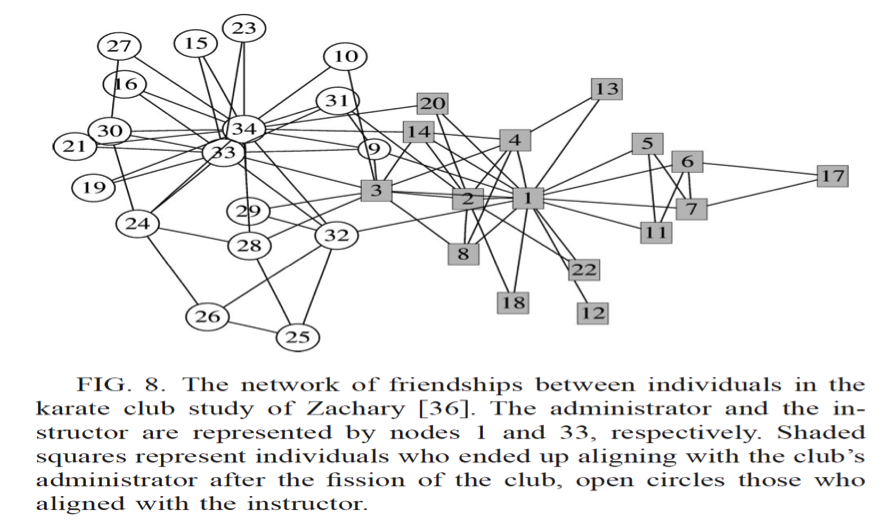
\includegraphics[keepaspectratio=true,scale=.8]{g1.png}}
\captionof{figure}{Zachary’s resulting split}% only if needed
\label{visina8}
\end{minipage}
\\
As a solution to determine if the split was predictable or not I used “igraph”; which is a collection of software packages for graph theory and network analysis. I downloaded the karate club data from the source file found at \url{http://igraph.sourceforge.net/karate.net}, and I took two approaches:
\subsection{ \huge Method One:}
\subsection*{ Algorithm name:}
Girvan Newman algorithm\\
It is one of the methods used to detect communities. The method focuses on the edges that are the least central. This method is preformed by removing edges from the graph until the graph is divided into different graphs.

\subsection*{The algorithm's steps:}
1-The betweenness of all existing edges in the network is calculated first.(the number of shortest paths between pairs of nodes that run along it)\\
2-The edge with the highest betweenness is removed.\\
3-The betweenness of all edges affected by the removal is recalculated.\\
4-Steps 2 and 3 are repeated until no edges remain.

\subsection*{Function used in R:}
edge.betweenness.community

\subsection*{R code:}

\begin{lstlisting}[language=R,frame=single]
# parts of the code was found at:
#http://igraph.wikidot.com/community-detection-in-r
library(igraph)
#downloading the data
g <- read.graph("~/Desktop/Assignment6/karate.net", format="pajek")
ebc <- edge.betweenness.community(g)
mods <- sapply(0:ecount(g), function(i) {
 g2 <- delete.edges(g, ebc$removed.edges[seq(length=i)])
 cl <- clusters(g2)
if(no.clusters(g2)==2){
plot(g2)
print(cl)}})
\end{lstlisting}
\newpage
\subsection*{The resulting output (from printing cl):}
\begin{lstlisting}[language=R,frame=single]
$membership
 [1] 1 1 2 1 1 1 1 1 2 2 1 1 1 1 2 2 1 1 2 1 2 1 2 2 2 2 2 2 2 2 2 2 2 2
$csize
[1] 15 19
$no
[1] 2
\end{lstlisting}

\subsection*{The resulting graph:}
\noindent
\begin{minipage}{\linewidth}
\fbox{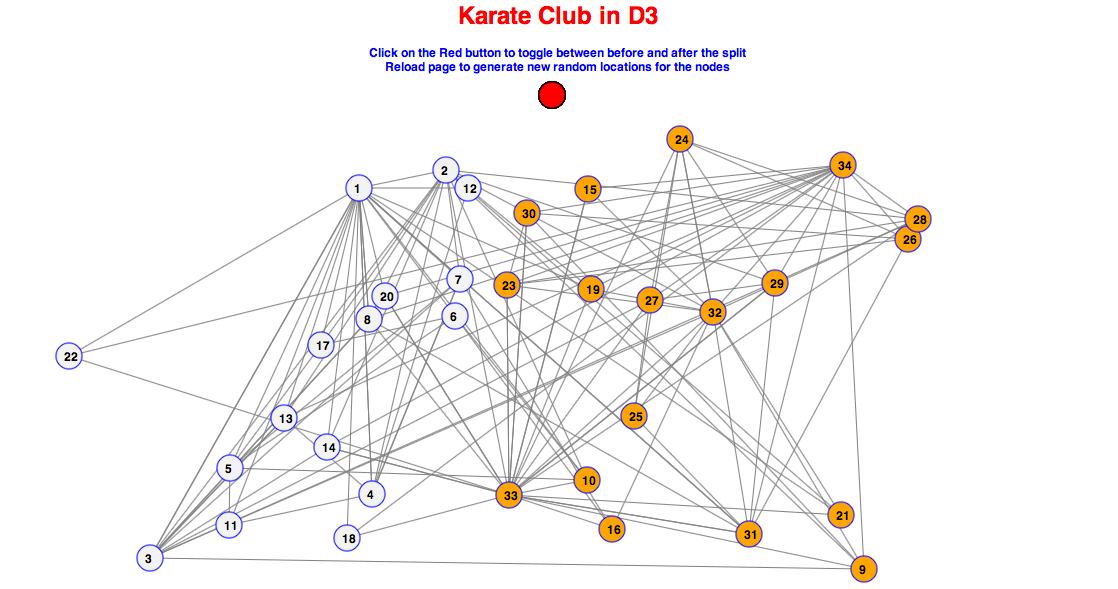
\includegraphics[keepaspectratio=true,scale=.8]{g2.png}}
\captionof{figure}{Predicted Split-Method One}% only if needed
\label{visina8}
\end{minipage}

\subsection*{Result:}
By comparing the existing split and the split we got from the code. We notice that node 3 was in group 1 in Zacharys split but it was in group2 in our predicted split.\\
\\
We compare the number of edges between the graph before and after the split (note that I split the graph to show each group separately)\\
\newpage
\begin{lstlisting}[language=R,frame=single]
> summary(g)
IGRAPH U--- 34 78 -- 
> summary(g2)
IGRAPH U--- 34 52 --
\end{lstlisting}

However, this method is slow there are 26 edges to be removed so total run time is O(26$^{2n}$).

The actual betweenness result is 6 different communities; in the code I limited it to 2 clusters and compared the resulting graph with Zacharys split.

\noindent
\begin{minipage}{\linewidth}
\fbox{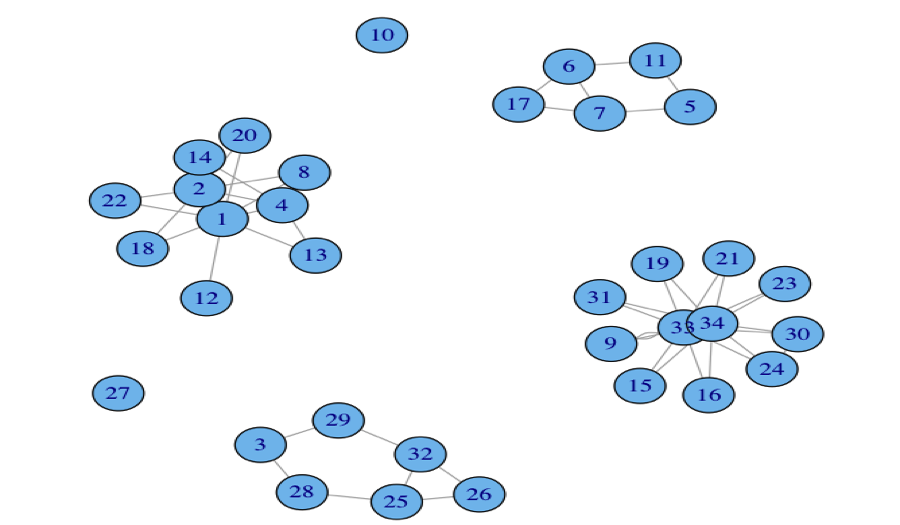
\includegraphics[keepaspectratio=true,scale=1]{g3.png}}
\captionof{figure}{Resulting Split}% only if needed
\label{visina8}
\end{minipage}

\begin{lstlisting}[language=R,frame=single]
> ebc
Graph community structure calculated with the edge betwenness algorithm
Number of communities (best split): 6 
Modularity (best split): 0.3850263 
Membership vector:
 [1] 1 1 2 1 3 3 3 1 4 5 3 1 1 1 4 4 3 1 4 1 4 1 4 4 2 2 6 2 2 4 4 2 4 4

> modularity(g, membership(ebc))
[1] 0.3850263
\end{lstlisting}


\newpage
\subsection{\huge Method Two:}
Algorithm name: leading eigenvector algorithm developed by Mark Newman.\\
This function tries to find densely connected subgraphs in a graph by calculating the leading non-negative eigenvector of the modularity matrix of the graph.

\subsection*{Algorithm Steps:}
Calculating the eigenvector of the modularity matrix for the largest positive eigenvalue and then separating vertices into two community based on the sign of the corresponding element in the eigenvector. If all elements in the eigenvector are of the same sign that means that the network has no underlying community structure.

\subsection*{Function used in R:}
leading.eigenvector.community 

\subsection*{R code:}

\begin{lstlisting}[language=R,frame=single]
#Parts of the code found at:
#http://igraph.sourceforge.net/screenshots2.html
library(igraph)
g <- read.graph("("~/Desktop/Assignment6/karate.net ",format="pajek")
cs<-leading.eigenvector.community(g,steps=1)
V(g)$color<-ifelse(cs$membership==1,"lightblue","green")
scale<-function(v,a,b){v<-v-min(v);v<-v/max(v);v<-v*(b-a);v+a}
#color
V(g)$size<-scale(abs(cs$eigenvectors[[1]]),10,20)
E(g)$color<-"grey"
E(g)[V(g)[color=="lightblue"]%--%V(g)[color=="green"]]$color<-"red"
#tkplot
tkplot(g,layout=layout.kamada.kawai,vertex.label.font=2)
\end{lstlisting}

\noindent
\begin{minipage}{\linewidth}
\fbox{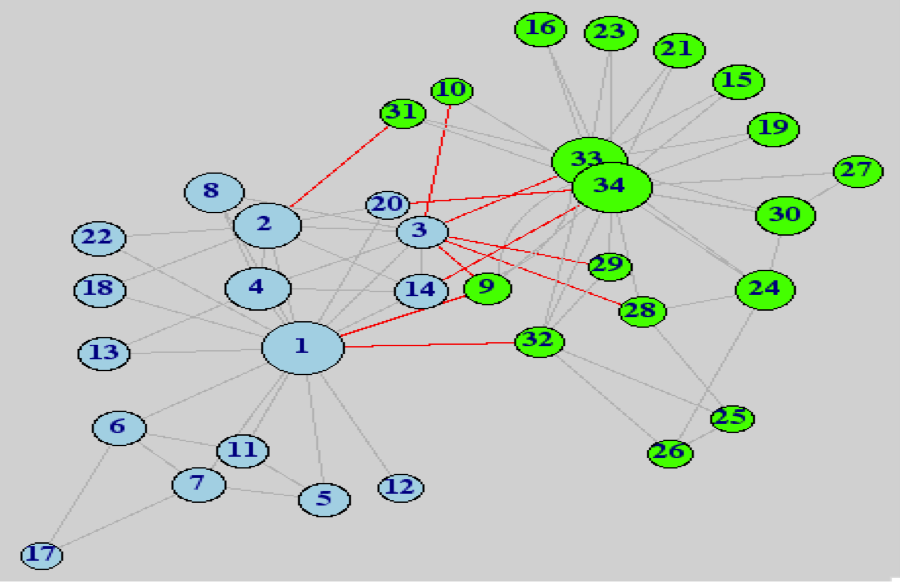
\includegraphics[keepaspectratio=true,scale=1]{g4.png}}
\captionof{figure}{Predicted Split-Method Two}% only if needed
\label{visina8}
\end{minipage}

\subsection*{Further Analysis:}

\begin{lstlisting}[language=R,frame=single]
> cs
Graph community structure calculated with the leading eigenvector algorithm
Number of communities (best split): 2 
Modularity (best split): 0.3714661 
Membership vector:
 [1] 1 1 1 1 1 1 1 1 2 2 1 1 1 1 2 2 1 1 2 1 2 1 2 2 2 2 2 2 2 2 2 2 2 2

> sizes(cs)
Community sizes
 1  2 
16 18

> modularity(g, membership(cs))
[1] 0.3714661
\end{lstlisting}

\subsection*{Result:}
When analyzing this graph and comparing it to the split that occurred, I found them to be exactly the same. So this method predicted the split one hundred percent.\\
\\
Also, I have noticed that the tkplot editor in R package is better than the X11 plot since you can move the nodes around to have a better view, however it is used for small graphs only. The editor tkplot is downloaded from: \url{http://cran.r-project.org/bin/macosx/tools/}
\\
\\
\uline{Other community detection algorithms:}\\
I have tested other community detection algorithm to see if any other algorithm predicted the same resulting split; and I got the following results.\\

\begin{itemize}
\item	walktrap.community\\
\begin{lstlisting}[language=R,frame=single]
> walktrap.community(g, modularity=TRUE)
Graph community structure calculated with the walktrap algorithm
Number of communities (best split): 5 
Modularity (best split): 0.3614399 
Membership vector:
 [1] 1 1 3 1 5 5 5 1 3 3 5 1 1 3 2 2 5 1 2 1 2 1 2 4 4 4 2 4 3 2 2 3 2 2
\end{lstlisting}
\item spinglass.community\\
\begin{lstlisting}[language=R,frame=single]
> spinglass.community(g, spins=10)
Graph community structure calculated with the spinglass algorithm
Number of communities: 4 
Modularity: 0.4160092 
Membership vector:
 [1] 2 2 2 2 3 3 3 2 1 1 3 2 2 2 1 1 3 2 1 2 1 2 1 4 4 4 1 4 4 1 1 4 1 1
\end{lstlisting}
\newpage
\item label.propagation.community\\
\begin{lstlisting}[language=R,frame=single]
> label.propagation.community(g)
Graph community structure calculated with the label propagation algorithm
Number of communities: 3 
Modularity: 0.3744247 
Membership vector:
 [1] 1 1 2 1 3 3 3 1 2 2 3 1 1 1 2 2 3 1 2 1 2 1 2 2 2 2 2 2 2 2 2 2 2 2
\end{lstlisting}
\item fastgreedy.community\\
\begin{lstlisting}[language=R,frame=single]
> fastgreedy.community(g)
Error in fastgreedy.community(g) : 
  At fast_community.c:552 : fast-greedy community finding works only on graphs without multiple edges, Invalid value
\end{lstlisting}
\ldots
\end{itemize}
\newpage

\section*{Extra Credit, 3 Points}

We know the group split into two different groups. Suppose the disagreements in the group were more nuanced -- what would the clubs look like if they split into groups of 3, 4, and 5?

\newpage

\section*{Answer to Extra Credit}
Different community algorithms split the initial graph to different number of community. And by knowing the resulting number of communities for each (shown at end of question one), I have selected the algorithms that result in 3, 4, and 5 number of groups.
\\
Also,the splits can be done as well by the same code used in question one, but changing the number of resulted clustering.\\

\subsection*{Three groups:}
\uline{R Code:}\\
\begin{lstlisting}[language=R,frame=single]
> G3 <- label.propagation.community(g)
> plot(G3,g,vertex.size=15,vertex.label.color= "black",vertex.label.cex=0.45,layout=layout.fruchterman.reingold)
\end{lstlisting}

\uline{The resulting graph:}\\
\\
\noindent
\begin{minipage}{\linewidth}
\fbox{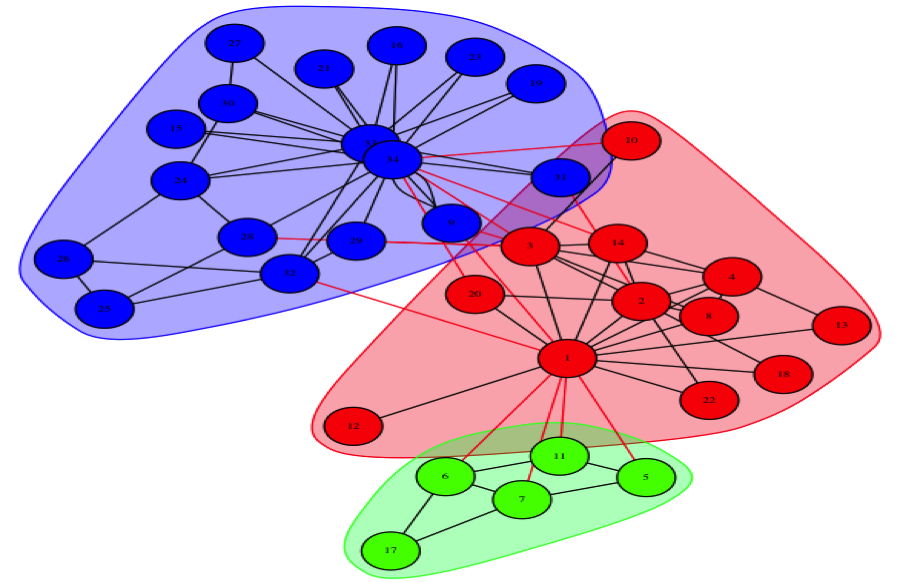
\includegraphics[keepaspectratio=true,scale=1]{g5.png}}
\captionof{figure}{Three Groups}% only if needed
\label{visina8}
\end{minipage}

\uline{R Code:}\\
\begin{lstlisting}[language=R,frame=single]
library(igraph)
#downloading the data
g <- read.graph("~/Desktop/Assignment6/karate.net", format="pajek")
ebc <- edge.betweenness.community(g)
mods <- sapply(0:ecount(g), function(i) {
 g2 <- delete.edges(g, ebc$removed.edges[seq(length=i)])
 cl <- clusters(g2)
if(no.clusters(g2)==3){
plot(g2)
print(cl)
}
})
\end{lstlisting}
\uline{The resulting graph:}\\
\noindent
\begin{minipage}{\linewidth}
\fbox{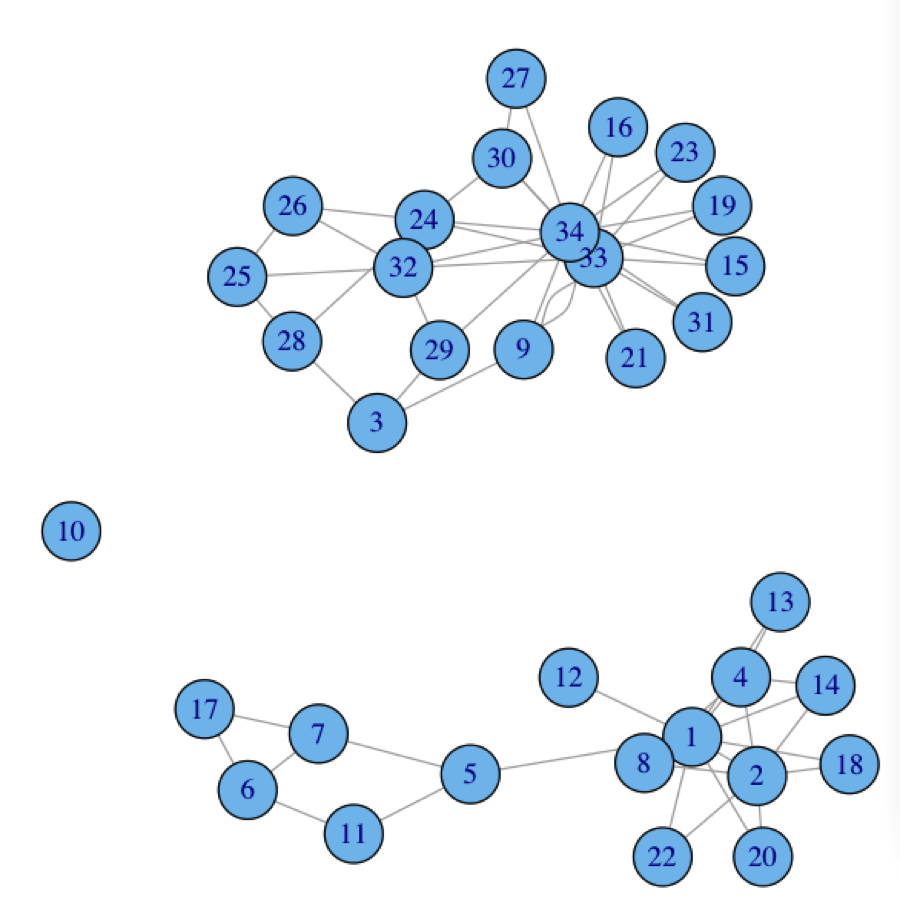
\includegraphics[keepaspectratio=true,scale=1]{g6.png}}
\captionof{figure}{Three Groups}% only if needed
\label{visina8}
\end{minipage}
\\
\newpage
\subsection*{Four groups:}
\uline{R code:}\\
\begin{lstlisting}[language=R,frame=single]
> G4 <- spinglass.community(g, spins=10)
> plot(G4,g,vertex.size=15,vertex.label.color= "black",vertex.label.cex=0.45,layout=layout.fruchterman.reingold)
\end{lstlisting}
\uline{The resulting graph:}\\
\noindent
\begin{minipage}{\linewidth}
\fbox{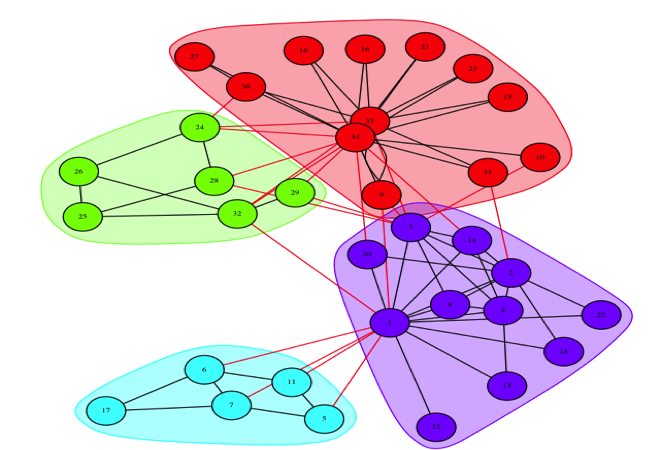
\includegraphics[keepaspectratio=true,scale=1]{g7.png}}
\captionof{figure}{Four groups}% only if needed
\label{visina8}
\end{minipage}
\newpage
\uline{R Code:}\\
\begin{lstlisting}[language=R,frame=single]
library(igraph)
#downloading the data
g <- read.graph("~/Desktop/Assignment6/karate.net", format="pajek")
ebc <- edge.betweenness.community(g)
mods <- sapply(0:ecount(g), function(i) {
 g2 <- delete.edges(g, ebc$removed.edges[seq(length=i)])
 cl <- clusters(g2)
if(no.clusters(g2)==4){
plot(g2)
print(cl)}
})
\end{lstlisting}

\uline{The resulting graph:}\\
\noindent
\begin{minipage}{\linewidth}
\fbox{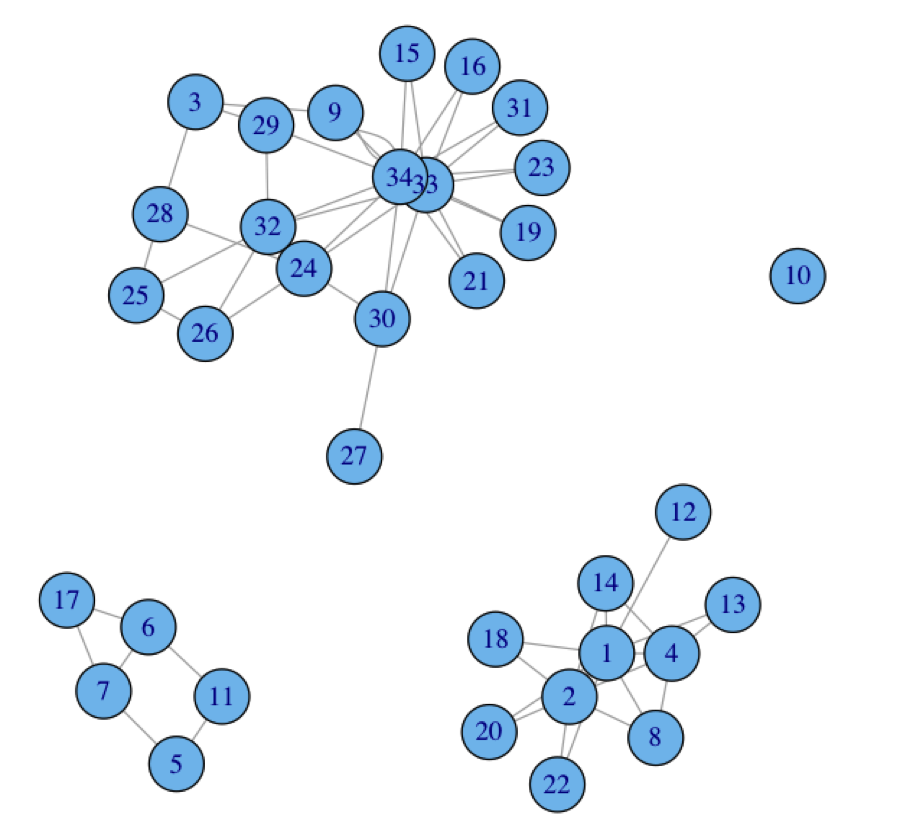
\includegraphics[keepaspectratio=true,scale=1]{g8.png}}
\captionof{figure}{Four groups}% only if needed
\label{visina8}
\end{minipage}
\newpage
\subsection*{Five groups:}
\uline{R Code:}\\
\begin{lstlisting}[language=R,frame=single]
> G5 <- walktrap.community(g, modularity=TRUE)
> plot(G5,g,vertex.size=15,vertex.label.color= "black",vertex.label.cex=0.45,layout=layout.fruchterman.reingold)
>mycolors <- heat.colors(length(G5))
tkplot(g, vertex.color=mycolors[membership(G5)])
\end{lstlisting}
\uline{The resulting graph:}\\
\noindent
\begin{minipage}{\linewidth}
\fbox{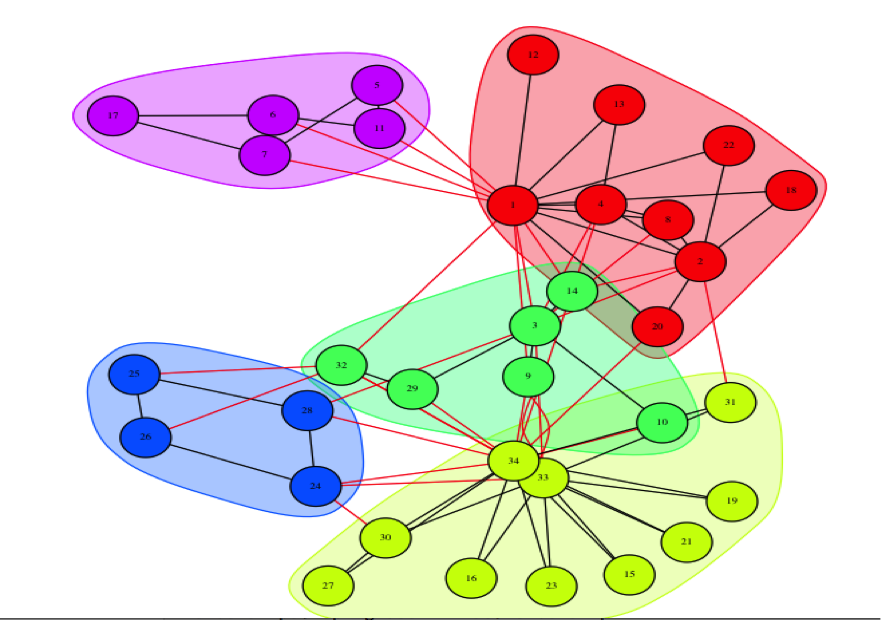
\includegraphics[keepaspectratio=true,scale=1]{g9.png}}
\captionof{figure}{Five Groups}% only if needed
\label{visina8}
\end{minipage}
\newpage
\uline{R Code:}\\
\begin{lstlisting}[language=R,frame=single]
library(igraph)
#downloading the data
g <- read.graph("~/Desktop/Assignment6/karate.net", format="pajek")
ebc <- edge.betweenness.community(g)
mods <- sapply(0:ecount(g), function(i) {
 g2 <- delete.edges(g, ebc$removed.edges[seq(length=i)])
 cl <- clusters(g2)
if(no.clusters(g2)==5){
plot(g2)
print(cl)}
})
\end{lstlisting}
\uline{The resulting graph:}\\
\noindent
\begin{minipage}{\linewidth}
\fbox{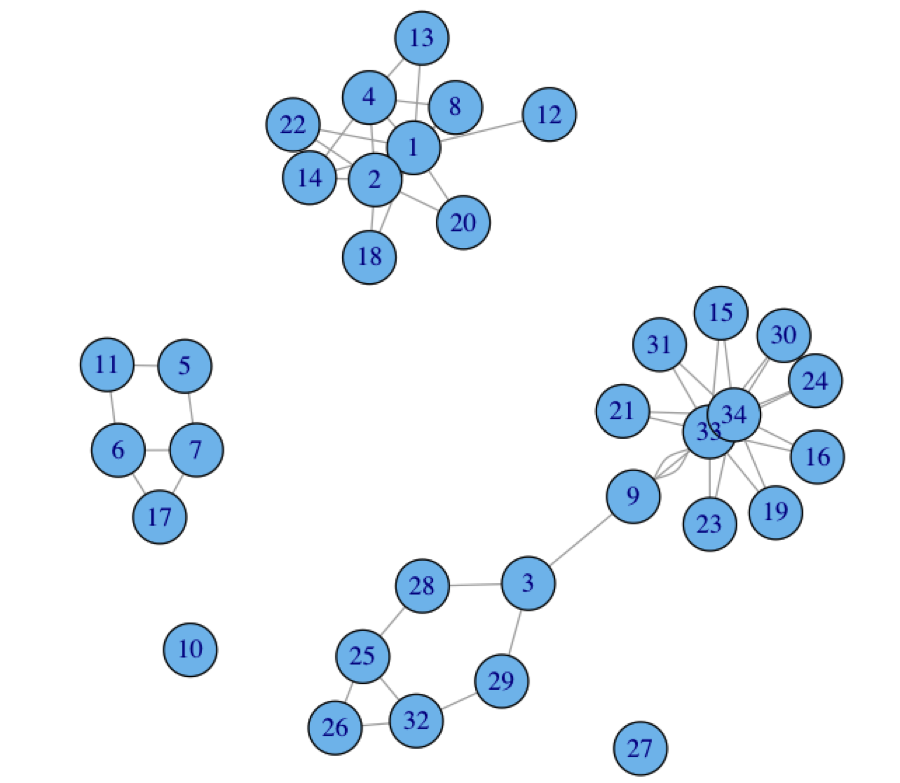
\includegraphics[keepaspectratio=true,scale=1]{g10.png}}
\captionof{figure}{Five Groups}% only if needed
\label{visina8}
\end{minipage}

\newpage
\section*{Reference}

\begin{itemize}

\item \url{http://aris.ss.uci.edu/~lin/76.pdf}
\item \url{http://www-personal.umich.edu/~ladamic/courses/networks/si614w06/ppt/lecture18.ppt}
\item \url{http://clair.si.umich.edu/si767/papers/Week03/Community/CommunityDetection.pptx}
\item \url{http://networkx.github.io/documentation/latest/examples/graph/karate_club.html}
\item \url{http://nbviewer.ipython.org/url/courses.cit.cornell.edu/info6010/resources/11notes.ipynb}
\item \url{http://stackoverflow.com/questions/9471906/what-are-the-differences-between-community-detection-algorithms-in-igraph/9478989#9478989}
\item \url{http://stackoverflow.com/questions/5822265/are-there-implementations-of-algorithms-for-community-detection-in-graphs}
\item \url{http://konect.uni-koblenz.de/networks/ucidata-zachary}
\item \url{http://vlado.fmf.uni-lj.si/pub/networks/data/ucinet/ucidata.htm#zachary}
\item \url{http://igraph.wikidot.com/community-detection-in-r}
\item \url{https://github.com/igraph/igraph/tree/master/interfaces/R/igraph/}
\item \url{http://books.google.com/books?id=atfCl2agdi8C&pg=PA70&lpg=PA70&dq=zachary+karate+club+predicted+split&source=bl&ots=LyTV0moGuw&sig=iOWdV68vQWRteDqJhCCuTO0usos&hl=en&sa=X&ei=GGtsUvG_NO-WyAHFm4GIDw&ved=0CDEQ6AEwAA#v=onepage&q&f=false}
\item \url{http://www.cs.cornell.edu/home/kleinber/networks-book/networks-book.pdf}
\item \url{http://theory.ic.ac.uk/7Etime/networks/communitystructure.html#louvain}
\item \url{http://igraph.sourceforge.net/doc-0.6/html/ch22s05.html}
\item \url{http://en.wikipedia.org/wiki/Girvan–Newman_algorithm}
\item \url{https://github.com/kjahan/community}
\item \url{http://www.cse.iitk.ac.in/users/sigml/slides/s01e02.pdf}
\item \url{http://igraph.sourceforge.net/doc/R/community.edge.betweenness.html}
\item \url{http://stackoverflow.com/questions/15787145/saving-the-plots-in-igraph-as-igraph-object-or-gml-format}
\ldots
\end{itemize}

\end{document}